% q0031.tex — The Visible Hand
\question{
  id        = {0031},
  title     = {The Visible Hand},
  source    = {OBECON},
  year      = {2026},
  round     = {Seletiva IEO -- Phase B},
  language  = {English},
  topic     = {Macro},
  subtopic  = {Coordination Games / Fiscal Policy / Big Push},
  type      = {dissertative},
  statement = {%
    Investment plays a crucial role in driving economic growth, but it is
    also the most volatile component of GDP, as illustrated in Figure~1.
    Unlike consumption or government spending, investment decisions often
    depend on expectations about what others will do, leading to strong
    complementarities and social interdependence.

    \begin{center}
    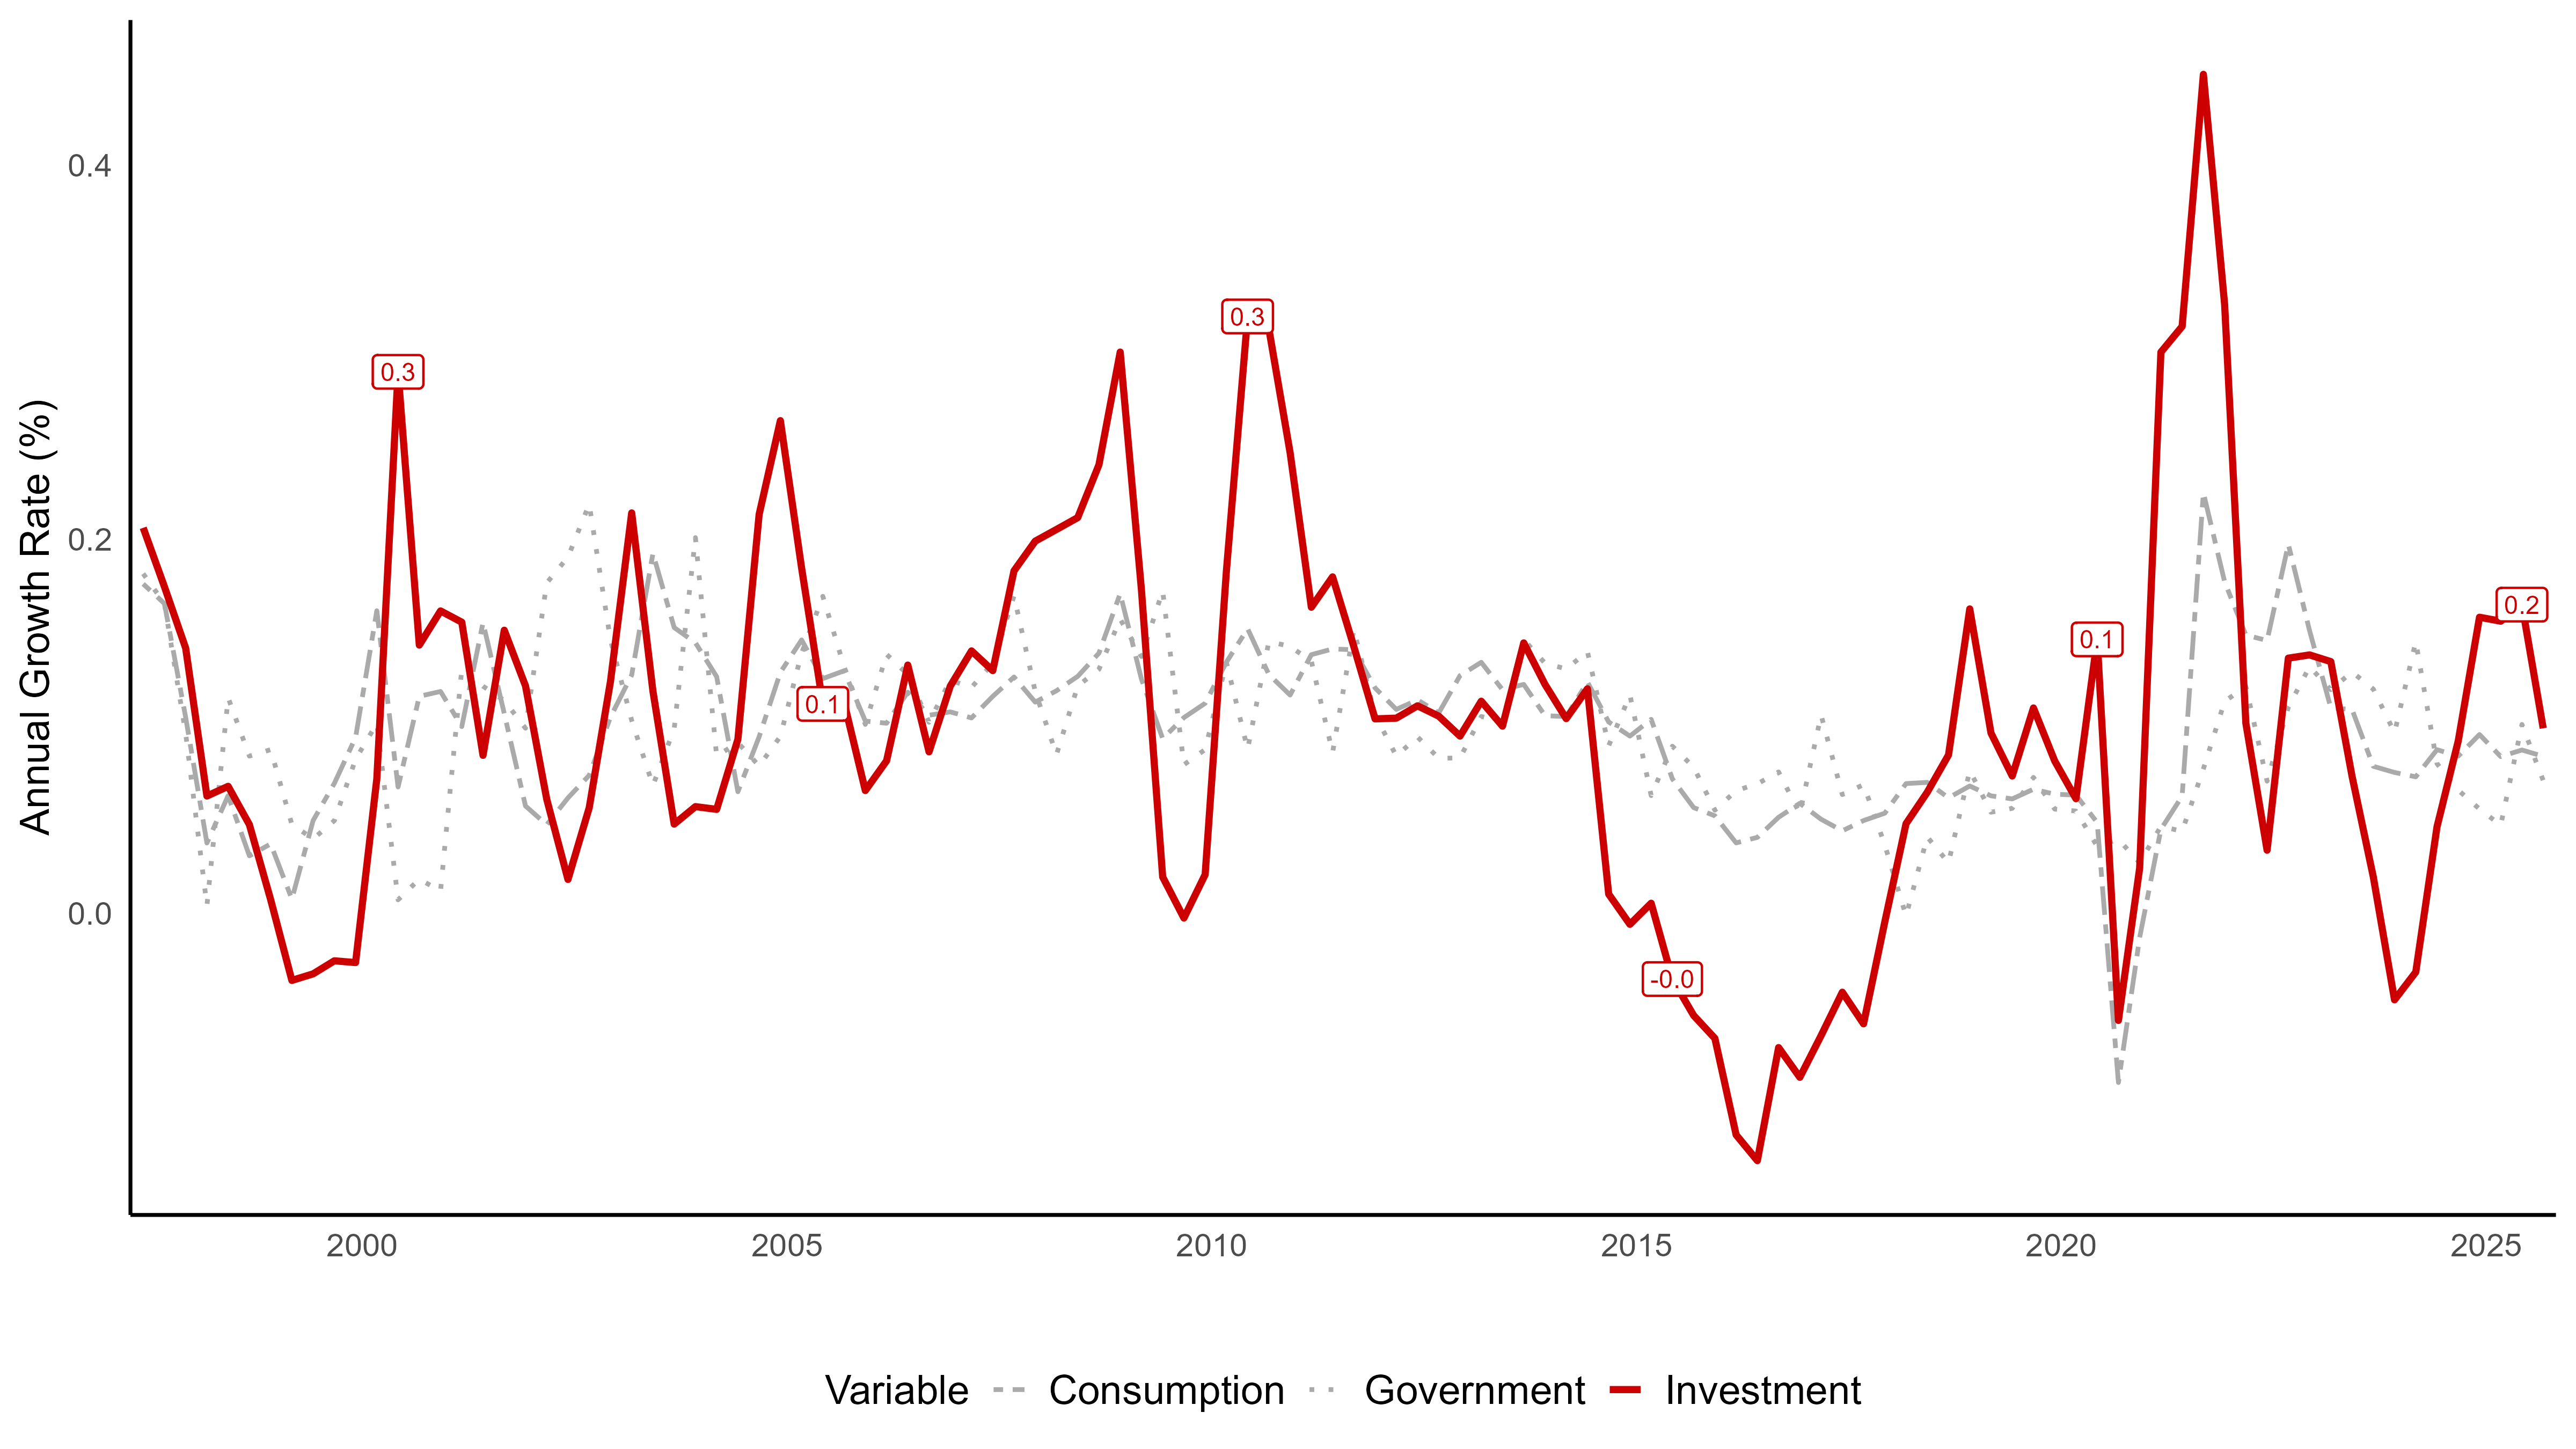
\includegraphics[width=0.85\textwidth]{../images/q0031_fig1.png}
    \end{center}

    Consider an economy with 250 identical private firms. Each firm~$i$
    simultaneously decides whether to invest ($I_i = 1$) or not invest
    ($I_i = 0$). Investing requires a private cost of~1. If a firm invests,
    it earns revenue
    \[
      R = \frac{2(P + G)}{250},
    \]
    where $P = \sum_{i=1}^{250} I_i$ is total private investment and $G$ is
    the government's public investment. A non-investing firm retains a
    current profit of~1.

    \begin{enumerate}[(a)]
      \item (25 points) In national accounts, what is included in
            ``Investment''? Give a concise definition and list the main
            categories.

      \item (25 points) Some theorists argue government spending can ``crowd
            out'' private investment. Briefly describe the mechanism.

      \item (25 points) Suppose $G = 0$.
            \begin{enumerate}[(i)]
              \item Show that \emph{all firms invest} ($I_i=1$ for all $i$)
                    is a Nash equilibrium.
              \item Show that \emph{no firm invests} ($I_i=0$ for all $i$)
                    is also a Nash equilibrium.
            \end{enumerate}

      \item (25 points) Now the government sets $G = 200$, financed by a
            lump-sum tax of \$0.80 on each firm.
            \begin{enumerate}[(i)]
              \item Show that \emph{all firms invest} is now the \textbf{unique}
                    Nash equilibrium.
              \item Interpret these results: what do they imply about
                    multiple equilibria, coordination failures, and the logic
                    of a ``big push''? Provide a brief policy implication.
            \end{enumerate}
    \end{enumerate}
  },
  choices   = {},
  answer    = {},
  solution  = {%
    \textbf{(a)} Investment (gross fixed capital formation plus inventory
    changes) covers: business machinery and equipment, non-residential
    structures, residential construction, intellectual property products
    (R\&D, software), and changes in inventories. Financial asset purchases
    are excluded.

    \textbf{(b)} Higher government borrowing absorbs scarce loanable funds,
    pushing up real interest rates and making private investment more
    expensive --- the classical crowding-out mechanism. Alternatively,
    higher taxes reduce after-tax returns to private investment.

    \textbf{(c.i)} If all firms invest, $P=250$ and the payoff to investing is
    $1 + 2(250)/250 - 1 = 2 > 1$ (payoff from not investing). No firm
    deviates.

    \textbf{(c.ii)} If no firm invests, $P=0$ and the payoff to a single
    deviating firm is $1 + 2(1)/250 - 1 = 2/250 < 1$. No firm deviates.

    \textbf{(d.i)} With $G=200$ and tax 0.8 per firm. Even if $k=0$ other
    firms invest, the payoff to investing is $0.2 + 2(201)/250 - 1 = 0.808 >
    0.2$ (payoff from not investing). Investing is a dominant strategy, so
    all-invest is the unique equilibrium.

    \textbf{(d.ii)} Without public investment the economy has two equilibria:
    a good one (all invest) and a bad one (no one invests). This is a
    coordination failure: even if the high-investment outcome is efficient,
    pessimistic expectations can trap the economy in the low-investment
    equilibrium. A sufficiently large public investment (``big push'')
    eliminates the bad equilibrium by making investment a dominant strategy,
    justifying temporary fiscal stimulus to coordinate private expectations.
  },
}
